\chptr{Meccanica}
\marginpar{\minitoc}

\section{Energia}
Con la cinematica abbiamo trattato unicamente il moto ``come appare'', slegato
dalle sue cause. Con la dinamica abbiamo invece introdotto quelle cause, ovvero le
forze. In questo capitolo effettuiamo un passo in più: Unendo
i concetti definiti fino ad ora, possiamo scoprire una quantità spesso
interpretata come il costo con il quale si pagano cambiamenti e trasformazioni
nell'universo: L'energia. Spiegare cosa sia l'energia valica il confine della
filosofia; la fisica contemporanea si limita a postulare l'esistenza di questa
quantità, misurabile indirettamente da altre quantità, che possiede la peculiare
caratteristica di conservarsi in sistemi isolati. In altre parole, se un
sistema non comunica in nessun modo con l'esterno, la quantità di energia di
quel sistema non cambia mai. Essa può al più trasformarsi e per questo
motivo non è un qualcosa di tangibile e direttamente osservabile; possiamo solo
vederne gli effetti. Questo perché l'energia viene sempre
definita attraverso altre proprietà ben riconoscibili: Distanze,
masse, lo scorrere del tempo. Moltiplicando, dividendo ed effettuando altre
operazioni (che definiremo) di queste quantità su un sistema, scopriremo che
il risutato che si ottiene è sempre lo stesso.

Quella della conservazione è una caratteristica che contraddistingue altre
quantità fisiche, tra le quali vedremo, nel prossimo capitolo, solo la quantità di moto


\section{Lavoro di una forza}
Precedentemente abbiamo introdotto
l'energia come un costo, che può essere convertito e speso per effettuare certi
cambiamenti in natura. Il lavoro di una forza è la forma di energia più familiare,
perché esprime il contributo di una forza allo spostamento di un oggetto, qualcosa
che associamo al moto e dunque ad un'espressione di ``vitalità'': Auto in movimento
mediante il motore,
una persona che cammina per mezzo della muscolatura, un oggetto in caduta libera a
causa del suo peso.

Il lavoro di una forza $\vecsymb{F}$ costante corrisponde al prodotto scalare\footnote{Ricordiamo
che il prodotto scalare $p$ tra due vettori $\vecsymb{a}$ e $\vecsymb{b}$ è un valore scalare
definito da $p = ab\cos\theta_{\vecsymb{ab}}$, con $\theta_\vecsymb{ab}$
l'angolo tra i vettori.}
tra la forza e lo spostamento $\vecsymb{s} = \Delta\vecsymb{r} = \vecsymb{r}_f - \vecsymb{r}_i$,
dove $\vecsymb{r}_i$ e $\vecsymb{r}_f$ sono vettori che descrivono rispettivamente
le posizioni iniziale e finale del punto materiale in moto:

\begin{align}
W \eqdef \vecsymb{F}\cdot\vecsymb{s}\label{workconstforce}
\end{align}

\noindent Il lavoro si misura in Joule (J), dove
\[ 1\text{ J} = 1\text{ Nm} = 1\text{ kg$\frac{\text{m}^2}{\text{s}^2}$} \]

La definizione \ref{workconstforce} presuppone che la forza $\vecsymb{F}$
rimanga sempre constante durante lo spostamento $\vecsymb{s}$. Questo non è
sempre vero nella realtà. Per questo possiamo definire il lavoro infinitesimo
nel seguente modo

\begin{align}
    dW \eqdef \vecsymb{F} \cdot d\vecsymb{s}\label{workvarforce}
\end{align}

\noindent dove supponiamo che per il tratto infinitesimo $d\vecsymb{s}$ agisca
una certa forza costante $\vecsymb{F}$. Se poi definiamo $\vecsymb{F}$ in
funzione dello spostamento, $\vecsymb{F}(\vecsymb{s})$, allora possiamo integrare
su tale funzione per ottenere il lavoro totale tra due coordinate $A,B$.

\begin{align}
    W_{AB} = \int_{A}^{B}\vecsymb{F}\cdot d\vecsymb{s}
\end{align}

\noindent Se si sviscera il prodotto scalare della definizione \ref{workvarforce},
otteniamo

\begin{align}
    dW = \vecsymb{F}\cdot d\vecsymb{s} = Fds\cos\theta\label{lavoroinfinitesimoangolo}
\end{align}

\noindent dove $\theta$ è l'angolo compreso tra i vettori $\vecsymb{F}$
e $\vecsymb{s}$. Notiamo che, per via del prodotto scalare, $dW$ è uno scalare, non un vettore, e
può essere positivo, negativo o nullo. A seconda del caso, il lavoro
viene in genere nominato come segue:

\begin{itemize}
    \item \textit{Lavoro motore:} $dW > 0$
    \item \textit{Lavoro resistente:} $dW < 0$ (la forza si oppone allo spostamento)
    \item \textit{Lavoro nullo:} $dW = 0$ (forza nulla o spostamento nullo o la forza è ortogonale allo spostamento): un
    esempio è la forza centripeta.
\end{itemize}

\subsection*{Osservazione ('importanza di scalare il Bondone)}
Quando si applica la definizione di lavoro in contesti pratici si può
giungere ad alcune osservazioni interessanti. Per esempio, avete mai
scalato il monte Bondone? Se la risposta è negativa, immaginate di
percorrere un sentiero che da Trento raggiunge la cima della montagna.
Durante la camminata, fatichiamo principalmente per due motivi: lo
sforzo dovuto allo spostamento orizzontale e quello impiegato per
salire di quota. Lo sforzo è indice del fatto che il nostro corpo
spende energia per muoversi e spostare la propria massa. Consideriamo
solamente il nostro peso, che è una forza che agisce in verticale e
che ci spinge verso il terreno. Proviamo a calcolare il
lavoro totale effettuato dal peso durante la camminata.
Purtroppo per noi, la nostra andatura è piuttosto irregolare:
percorriamo tratti in orizzontale, piccole discese e grandi
salite. Come al solito, la soluzione è ragionare all'infinitesimo:
dividiamo il nostro percorso in piccolissimi spostamenti $d\vecsymb{s}$,
sui quali agisce il peso $\vecsymb{P}$. Ricordando la definizione
\ref{lavoroinfinitesimoangolo}, il lavoro infinitesimo che $\vecsymb{P}$
effettua sul generico tratto $d\vecsymb{s}$ è

\[ dW = P ds \cos\theta \]

\noindent Il termine $ds \cos\theta$ è la proiezione del vettore
$d\vecsymb{s}$ sul vettore $\vecsymb{P}$, cioè la componente
parallela al peso. Dal momento che il peso punta sempre verso il
basso, ciò significa che eventuali spostamenti orizzontali (o in
generale la componente orizzontale di ogni spostamento) non
contribuiscono al lavoro del peso, perché i loro vettori sono
tra loro ortogonali. Da qui concludiamo che lo spostamento
che si deve considerare per il calcolo del lavoro è solamente
quello verticale $dh = ds \cos\theta$.

\[ W = \int_{h_\text{Trento}}^{h_\text{Bondone}} Pdh = \int_{h_\text{Trento}}^{h_\text{Bondone}} -mg dh = -mg(h_\text{Bondone} - h_\text{Trento}) \]

Ma questo non contraddice la nostra esperienza? Davvero è
questa l'energia che spendiamo per scalare il Bondone,
indipendentemente da quanto ci muoviamo in orizzontale? In realtà
il lavoro che abbiamo calcolato è il lavoro della forza peso, non
il lavoro che noi abbiamo speso per camminare e salire. Noi non
produciamo la forza peso e sono i nostri muscoli a contrapporsi
ad essa. Ovviamente anche la muscolatura compie del lavoro a livello
microscopico per spostarci in giro e noi sentiamo proprio questa fatica, anche
per spostamenti orizzontali.

%\subsubsection*{Versore}
%\[ \hat{v} = \frac{\overrightarrow{v}}{|\overrightarrow{v}|} \]
%\[ W = \int_{i}^{f}\overrightarrow{F}\cdot d\overrightarrow{s} = \int_{0}^{L}(F\hat{f})\cdot(ds\hat{x}) = F(\hat{f}\cdot\hat{x})\int_{0}^{L}ds = F\cos(\theta) L\]
%Quindi
%\[ \cos\theta = \frac{W}{FL} \]







\section{Il teorema delle forze vive}
L'ipotesi fondamentale per giungere all'enunciato del teorema
è la seconda legge della dinamica, oltre alla definizione di lavoro.
Supponiamo che $\vecsymb{F}$ sia una forza totale esercitata su
di un corpo di massa $m$. L'azione di $\vecsymb{F}$ produce uno
spostamento, che considereremo infinitesimo in modo da generalizzare
il ragionamento a forze variabili e dipendenti dallo spostamento
stesso. Allora

\[ \vecsymb{F} = m\frac{d\vecsymb{v}}{dt} \]

\noindent Senza giustificare le ragioni matematiche dei prossimi passaggi, ma facendoci
guidare dall'intuizione fisica, eseguiamo il prodotto scalare con $d\vecsymb{s}$
su entrambi i membri
\[ \vecsymb{F}\cdot d\vecsymb{s} = m\frac{d\vecsymb{v}}{dt}\cdot d\vecsymb{s} = m d\vecsymb{v}\cdot\frac{d\vecsymb{s}}{dt} \]
Notiamo che questa operazione ha permesso di ottenere un lavoro al membro di
sinistra, mentre a destra si ottiene il termine $d\vecsymb{s}/dt$, che corrisponderebbe
proprio alla velocità $\vecsymb{v}$. Con ulteriori sviluppi, si raggiunge la
seguente equazione (il simbolo $d$ ha il significato fisico di variazione o
differenza infinitesima).
\[ \vecsymb{F}\cdot d\vecsymb{s} = m\vecsymb{v}\cdot d\vecsymb{v} = m\text{ }d\left[\frac{v^2}{2}\right] \]
Dimostriamo come sviluppare il termine $\vecsymb{v}\cdot d\vecsymb{v} = d\left[\frac{v^2}{2}\right]$.
Ricorriamo alla definizione vettoriale di prodotto scalare\footnote{Il prodotto scalare
di due vettori $\vecsymb{a}$ e $\vecsymb{b}$ è calcolabile anche attraverso la somma
dei prodotti tra i valori delle componenti dei due vettori: $\vecsymb{a}\cdot\vecsymb{b} = a_xb_x + a_yb_y + ...$}
e utilizziamo questo abuso di notazione, ma ragionevole dal punto di vista fisico:
\[ \int x \,dx =  \frac{x^2}{2} + c \Rightarrow \frac{d}{dx}\left[\frac{x^2}{2} + c\right] = x \Rightarrow \int x \,dx = \int d\left[\frac{x^2}{2}\right] \]
Quindi
\[ v_x dv_x + v_y dv_y + v_z dv_z \Rightarrow d\left[\frac{v_x^2}{2}\right] + ... = d\left[\frac{v_x^2 + ...}{2}\right] = d\left[\frac{v^2}{2}\right] \]
Riprendendo l'equazione $\vecsymb{F}\cdot d\vecsymb{s} = m\text{ }d\left[\frac{v^2}{2}\right]$ otteniamo
\[ dW = d\left[\frac12 mv^2\right] \]
Il termine $E_K = \frac{1}{2}mv^2$ viene chiamato \textit{energia cinetica}. Quindi
\[ dW = dE_K \]
Questa equazione può essere tradotta come ``una infinitesima quantità di lavoro
corrisponde ad una variazione infinitesima dell'energia cinetica''. Ora possiamo
enunciare il teorema delle foze vive:
\vspace{8pt}
\begin{tcolorbox}[colback = red!30, colframe = red!30!black, title = {Teorema dell'energia cinetica (o delle forze vive)}]
    Quando una forza (risultante) applicata a un oggetto per un dato tratto di
    traiettoria, compie su di esso un lavoro, il risultato è una variazione del
    modulo della velocità dell'oggetto e quindi una variazione della sua energia
    cinetica. Quindi, il lavoro compiuto su un oggetto è uguale alla variazione
    della sua energia cinetica.
    \begin{align}
        W_{i\to f}^{(R)} = \Delta E_K\label{forzevive}
    \end{align}
\end{tcolorbox}
\vspace{5pt}

\noindent È necessario sottolineare alcune osservazioni:
\begin{enumerate}
    \item Il teorema presuppone che il lavoro sia dovuto all'effetto della risultante delle forze agenti sul corpo.
    \item Il lavoro è rappresentato da una variazione di energia cinetica. Possiamo descrivere dunque lo stato finale
    come \[ E_{K,f} = E_{K,i} + W_{i\to f} \] dunque se il lavoro, quindi l'energia trasferita all'oggetto, è positivo,
    l'energia cinetica aumenta e viceversa.

    \item Il teorema sposta la descrizione del sistema fisico dal piano vettoriale a quello scalare. Ovvero, partendo
    da grandezze vettoriali, abbiamo ottenuto una legge dove compaiono solamente dei numeri. Ciò rende particolarmente agevole
    l'utilizzo del teorema in svariati problemi nei quali l'analisi vettoriale può essere ostica.

    \item Il teorema è molto potente per la sua validità generale, perché non sono state fatte ipotesi sulla natura delle
    forze, se non presupponendo come vera la seconda legge della dinamica $\vecsymb{F} = m\vecsymb{a}$.
    La legge può essere dunque applicata ad un pendolo, ad una palla da bowling,
    a delle molecole microscopiche in movimento.
\end{enumerate}

\section*{Teorema delle forze vive (fato ben)}
Come adesso scopriremo, la definizione del lavoro introduce una
quantità fisica estremamente utile nella trattazione di fenomeni
di natura meccanica. Un risultato molto importante in merito è
il \textit{teorema dell'energia cinetica} (o, come un tempo,
\textit{delle forze vive}, da \textit{vis viva}).

Riprendiamo il secondo principio della dinamica

\[ \vecsymb{F} = m \vecsymb{a} = m \frac{d\vecsymb{v}}{dt} \]



\[ \vecsymb{F} \cdot d\vecsymb{s} = m \frac{d\vecsymb{v}}{dt} \cdot d\vecsymb{s} \]

\noindent dove al memobro di sinistra abbiamo ottenuto il lavoro
infinitesimale corrispondente, $dW$. Osserviamo tuttavia che
al membro di destra vale

\[ m d\vecsymb{v} \cdot \frac{d\vecsymb{s}}{dt} = m d\vecsymb{v} \cdot \vecsymb{v} \]

\noindent per definizione di velocità (istantanea). Osserviamo
dunque ciò che accade passando all'integrazione:

\[ \int_{i}^{f} m \vecsymb{v} \cdot d\vecsymb{v} = m \left[\frac{v^2}{2}\right]_{i}^{f} \]

\noindent Per questo ultimo passaggio, abbiamo fatto ricorso alla
definizione di prodotto scalare e alle proprietà degli integrali:

\[ \int \vecsymb{v} \cdot d\vecsymb{v} = \int v_x dv_x + v_y dv_y + ... = \frac{v_x^2}{2} + \frac{v_y^2}{2} + ... = \frac{v^2}{2} \]

\noindent Abbiamo dunque mostrato che

\[ W_{i \to f} = \frac{1}{2}mv_f^2 - \frac{1}{2}mv_i^2 \]

\noindent ovvero il lavoro totale (derivante cioè dalla risultante
$\vecsymb{F}$ su $m$, come avevamo supposto), dipende solo da
certe quantità che definiscono l'oggetto prima e dopo lo spostamento
nel quale ha agito la forza. La quantità $\frac12mv^2$ corrisponde
dimensionalmente ad una certa energia e viene definita
\textit{energia cinetica}

\[ E_K \stackrel{\text{def}}{=} \frac{1}{2}mv^2 \]

\noindent e rappresenta l'energia che un corpo possiede in
virtù del suo stato di moto, dunque della sua velocità ad un
certo istante.



%\subsubsection*{Applicazione del teorema delle forze vive}
%\textit{Supponiamo di avere un punto di massa $m$ sulla sommità di un piano
%inclinato di alteza $h$ con un angolo $\theta$ rispetto all'orizzontale. Sappiamo
%che la massa parte dalla cima con velocità $v_i$ parallela alla lunghezza del piano
%e diretta verso la discesa. Vogliamo trovare la velocità finale della massa. Si
%esprima il calcolo sia con che senza attrito, considerando nell'ultimo caso un
%coefficiente di attrito dinamico $\mu$.}
%\begin{marginfigure}
%    \centering
%    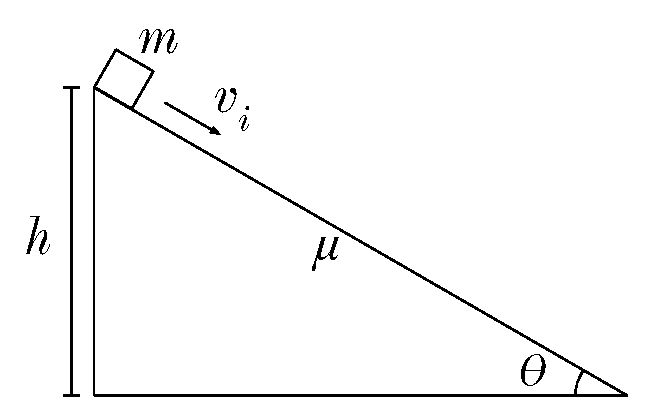
\includegraphics[width = \marginparwidth]{pianoinclinato.pdf}
%    \caption{Un piano inclinato}
%\end{marginfigure}
%\\\\
%Possiamo risolvere il problema utilizzando il teorema delle forze vive.
%\[ W = \Delta E_K \]
%\[ W = \vecsymb{P}\cdot\vecsymb{L} = |\vecsymb{P}||\vecsymb{L}|\cos\left(\frac{\pi}{2} - \theta\right) = |\vecsymb{P}||\vecsymb{L}|\sin\theta = |\vecsymb{P}|h = mgh \]
%\[ \Delta E_K = \frac12mv_f^2 - \frac12mv_i^2 \]
%Quindi
%\[ mgh = \frac12mv_f^2 - \frac12mv_i^2 \]
%\[ v_f = \sqrt{2gh + v_i^2} \]
%
%Con attrito il peso è contrastato. L'attrito compie il suo lavoro per tutta la
%lunghezza del piano fino alla fine della discesa. L'espressione della differenza
%di energia cinetica è tuttavia la stessa.
%\[ W = W_P - W_A = Ph - F_AL = Ph - \mu F_\perp L = mgh - \mu mg\sin\theta L \]
%
%
%\subsubsection*{Problemino}
%Supponiamo di avere un piano inclinato, con attrito e lunghezza $l$, come nel problema precedente.
%La massa viene stavolta lanciata con una velocità iniziale dalla base del piano.
%La massa raggiunge una certa altezza $h$ e poi scivola di nuovo fino in fondo. Si
%vuole determinare la velocità alla quale la massa raggiunge nuovamente la base del
%piano.

\section{Forze conservative}
In fisica, possiamo classificare le forze in \textit{conservative} e \textit{non
conservative}. La distinzione tra di esse sta nel fatto che quando agisce una
forza conservativa, il lavoro compiuto viene immagazzinato in una forma di energia,
\textit{l'energia potenziale}, che è possibile risprigionare. Il lavoro compiuto
da una forza non conservativa, invece, non può essere recuperato in seguito come
energia cinetica, ma viene trasformato in altre forme di energia. Le differenze tra
forze conservative e non conservative emergono se prendiamo in esame il moto di un
oggetto lungo una traiettoria chiusa.

\vspace{8pt}
\begin{tcolorbox}[colback = red!30, colframe = red!30!black, title = {Forza conservativa (condizione I)}]
    Una forza conservativa è una forza che compie un lavoro totale nullo lungo ogni
    percorso chiuso. Se il percorso è $\gamma = A\to A$ (il percorso si chiude su
    se stesso) e $\vecsymb{F}$ è una forza conservativa, allora:
    \begin{align}
        W_{A \to A} = \oint_\gamma \vecsymb{F} \cdot d\vecsymb{s} = 0 \qquad \forall \gamma
    \end{align}
\end{tcolorbox}
\vspace{5pt}

\noindent Da questa prima caratteristica delle forze conservative ne segue nua
seconda. Si considerino i percorsi tra $A$ e $B$ in Figura \ref{percorsi}.
\begin{marginfigure}
    \centering
    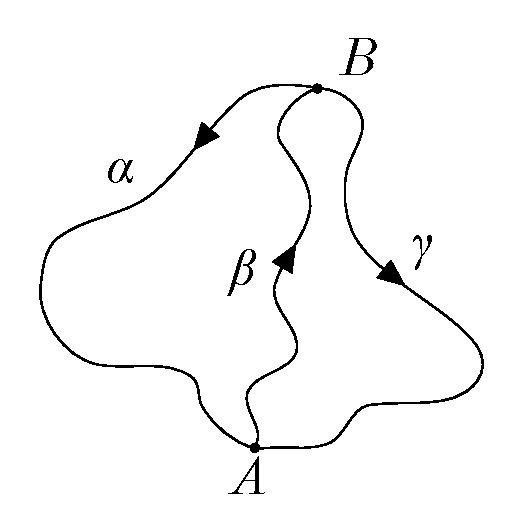
\includegraphics[width = \marginparwidth]{circ.pdf}
    \caption{Percorsi tra due punti in presenza di una forza conservativa}
    \label{percorsi}
\end{marginfigure}
Supponiamo di dover raggiungere il punto $A$ partendo da $B$ e possiamo fare
ciò percorrendo due strade differenti, $\alpha$ e $\gamma$. Disegnamo poi un
terzo percorso, che invece riporta $A$ in $B$.
Per ipotesi vale la condizione I, ovvero sta agendo una forza conservativa
lungo tali percorsi. Dunque, il lavoro compiuto dalla forza nei percorsi chiusi
$\alpha\beta$ e $\beta\gamma$ è nullo:
\begin{align*}
    W_{\alpha\beta} = W_\alpha + W_\beta = 0\\
    W_{\beta\gamma} = W_\beta + W_\gamma = 0
\end{align*}
Ma allora
\[ W_\beta = -W_\alpha = -W_\gamma \quad \therefore \quad W_\alpha = W_\gamma \]
Abbiamo mostrato che il lavoro compiuto dalla forza conservativa dal punto $B$
al punto $A$ è uguale per entrambi i percorsi. In altre parole, il lavoro totale
dipende solo dai punti $A$ e $B$.

Possiamo dimostrare questa proprietà in un altro modo. Consideriamo il percorso
chiuso $\beta\gamma$. Vale per ipotesi
\[ W_{\alpha\beta} = W_\beta + W_\gamma = \int_{A}^{B}\vecsymb{F}\cdot d\vecsymb{s} + \int_{B}^{A}\vecsymb{F}\cdot d\vecsymb{s} = 0 \]
Quindi 
\[ \int_{A}^{B}\vecsymb{F}\cdot d\vecsymb{s} = - \int_{B}^{A}\vecsymb{F}\cdot d\vecsymb{s} = \int_{A}^{B}\vecsymb{F}\cdot d\vecsymb{s} \]

\vspace{8pt}
\begin{tcolorbox}[colback = red!30, colframe = red!30!black, title = {Forza conservativa (condizione II)}]
    Una forza è conservativa se il lavoro totale compiuto da essa durante uno spostamento
    da $A$ a $B$ dipende unicamente da questi punti di partenza e di arrivo, non
    dal percorso seguito tra essi.
    \[ W[\vecsymb{F}]_{A\to B} \text{ indipendente dai percorsi tra A e B} \]
\end{tcolorbox}
\vspace{5pt}

\section{Energia potenziale}
Una forza conservativa può essere caratterizzata da una terza condizione che deriva
dalla seconda.

\vspace{8pt}
\begin{tcolorbox}[colback = red!30, colframe = red!30!black, title = {Forza conservativa (condizione III)}]
    Una forza è conservativa se il lavoro effettuato da essa è esprimibile in
    funzione delle sole ``coordinate'' $A$ e $B$ tramite una primitiva nella forma
    seguente:
    \[ W_{A\to B} = -\left[\mathcal{U}(\vecsymb{x}_B) - \mathcal{U}(\vecsymb{x}_A)\right] = -\Delta\mathcal{U} \]
\end{tcolorbox}
\vspace{5pt}

\noindent La differenza $\Delta\mathcal{U}$ viene chiamata differenza
di potenziale.

Questa condizione esprime la proprietà delle forze conservative di
consentire agli oggetti ad essa sottoposti di immagazzinare una certa quantità
di energia da essa trasferita se l'oggetto passa da $A$ a $B$ e di liberare
quella stessa energia nel tragitto inverso. Immaginiamo di lanciare una palla
nel vuoto. La forza peso, derivante dalla gravità, è conservativa. Mentre la
palla cade, il peso effettua un lavoro su di essa e di fatto la sua energia
cinetica aumenta. Quella energia deve pur provenire da qualche parte. Se osserviamo
questo esperimento ``invertendo il tempo'' (o equivalentemente lanciamo in alto
la palla), osseviamo che la forza peso esegue un lavoro negativo sulla palla,
quindi la sua energia cinetica diminuisce mano a mano. Ma il peso è una forza
conservativa, dunque l'energia da essa sottratta viene comunque conservata
in qualche forma. Questa è l'energia potenziale, che dipende appunto dalla differenza
di quota della palla.

Mostriamo come ricavare la condizione III. Sappiamo che il lavoro di una
forza conservativa è definita da un integrale, che non dipende dal percorso
effettuato tra l'inizio $A$ e la fine $B$. Dunque il lavoro deve in qualche modo
poter essere descritto da una funzione nelle variabili $A$ e $B$.
\[ W_{A \to B} = \int_{A}^{B}\vecsymb{F}\cdot d\vecsymb{s} = f(A,B) \]
Questa funzione sarà una qualche primitiva della funzione integranda, che sarà
quindi composta da dei contributi lineari di $A$ e $B$ dentro qualche funzione
$\mathcal{U}$ (a meno di costanti moltiplicative esterne alla funzione).
Abbiamo quindi le seguenti scelte:
\begin{align*}
    \mathcal{U}(A) + \mathcal{U}(B)\\
    \mathcal{U}(A) - \mathcal{U}(B)
\end{align*}
Ma sapendo che la funzione $f(A,B)$ è una qualche primitiva, ciò significa che
deve valere la proprietà di antisimmetria (invertendo gli estremi di integrazione,
deve cambiare il segno). Questa proprietà vale solo per la seconda funzione:
\[ f(B,A) = \mathcal{U}(B) - \mathcal{U}(A) = - (\mathcal{U}(A) - \mathcal{U}(B)) \]
Definiamo dunque la \textit{differenza di energia potenziale} per forze conservative.
\[ \Delta\mathcal{U}_{A\to B} = \mathcal{U}(B) - \mathcal{U}(A) = -W_{A\to B} \]
Notare che stiamo definendo solo la differenza di energia potenziale, non l'energia
potenziale in sé. Possiamo infatti fissare lo ``zero'' dell'energia potenziale in
modo del tutto arbitrario, in quanto esso non sarà mai utile nel risultato finale
di un problema di meccanica.

\subsection{Energia potenziale gravitazionale}
\subsection{Energia potenziale elastica}

\section[Conservazione]{Conservazione dell'energia meccanica}
Ricordiamo il teorema delle forze vive (Equazione \ref{forzevive})

\[ W = E_{K,f} - E_{K,i} \]

\noindent dove $W$ corrisponde al lavoro \textit{totale} delle forze
che agiscono sul corpo tra i momenti $i$ e $f$.
Abbiamo inoltre mostrato che il lavoro dovuto alle forze conservative ($\mathfrak{C}$)
è legato ad una differenza di energia potenziale:

\[ W_\mathfrak{C} = -(\mathcal{U}_f - \mathcal{U}_i) \]

\noindent Per il principio di sovrapposizione, possiamo esprimere il lavoro totale
nel seguente modo, separando l'insieme forze conservative $\mathfrak{C}$ e non conservative $\mathfrak{N}$:

\[ W = W_\mathfrak{C} + W_\mathfrak{N} \]

\noindent Unendo le equazioni finora ottenute,
\begin{align}
    W_\mathfrak{N} = \Delta E_K + \Delta\mathcal{U} = (E_{K,f} + \mathcal{U}_f) - (E_{K,i} + \mathcal{U}_i) = \Delta E\label{nonconserva}
\end{align}

\noindent Abbiamo unito quantità relative a momenti correlati,
cioè abbiamo unito energia cinetica finale con energia potenziale finale
ed energia cinetica iniziale con energia potenziale iniziale.
La somma di queste quantità viene chiamata \textit{energia meccanica}:
\begin{align}
    E \eqdef E_K + \mathcal{U}
\end{align}
Dalla \ref{nonconserva} possiamo notare che, se agiscono forze non conservative,
la variazione di energia meccanica corrisponde al lavoro effettuato dalle
froze non conservative stesse. Per questo, è intuitivo utilizzare l'equazione
nella forma
\[ E_f = E_i + W_\mathfrak{N} \]
perché permette di capire che l'energia meccanica finale del sistema cambierà
da quella iniziale di una certa quantità dovuta all'azione delle forze non
conservative, che possono aggiungere o sottrarre energia meccanica.
In assenza di forze non conservative, o in casi in cui le forze non
conservative si annullano, allora $W_\mathfrak{N} = 0$.
Segue dunque un importante teorema, ovvero il teorema di conservazione
dell'energia meccanica, che abbiamo appena dimostrato.

\vspace{8pt}
\begin{tcolorbox}[colback = red!30, colframe = red!30!black, title = {Teorema di conservazione dell'energia meccanica}]
    Se su un oggetto il lavoro totale delle forze non conservative è nullo,
    allora la sua energia meccanica si conserva.
    \begin{align}
        \Delta E = 0
    \end{align}
\end{tcolorbox}
\vspace{5pt}


\section{Approfondimenti}
Anche la meccanica è un intero multiverso di possibilità, leggi e
applicazioni affascinanti ma assai più complesse di come è stato
spiegato qui. Includiamo qualche approfondimento del quale è stata
proferita parola durante le lezioni.

\subsection{Perché ``forze vive''?}
Il lavoro di una forza è ben visibile quando esso agisce su un corpo
in movimento. Prendiamo l'esempio di un razzo che viene lanciato verso
il cielo: La propulsione data dal
propellente spinge il razzo verso l'alto e in termini sempliciotti lo
``aiuta'' a guadagnare velocità durante la salita, perché la forza è
concorde con lo spostamento (entrambi i vettori puntano verso l'alto
perpendicolarmente al terreno) e compie lavoro motore. Quando il razzo raggiunge la sua altezza
massima, in genere comincia a cadere, ma supponiamo che ad un certo
punto esso liberi un paracadute. La resistenza data dal paracadute
determina una forza che si oppone alla caduta del razzo; dunque, in
questo secondo caso, la resitenza dell'aria che gonfia il paracadute
compie un lavoro resistente, che si oppone al moto di caduta e per questo
frena il razzo e ne riduce la velocità.

Agli albori della meccanica ci si sarebbe riferiti all'effetto di queste
forze in gioco come \textit{vis viva}, o forza viva, una quantità o
un'essenza dotata di vita propria,
che trasferendosi da corpo a corpo determinava cambiamenti nello stato
di moto di quegli stessi corpi. Per tale ragione storica, il teorema
porta ancora in sé il termine di forza viva, anche se la fisica
contemporanea propende sempre più verso la denominazione di
\textit{teorema dell'energia cinetica}.